

%% bare_conf_compsoc.tex
%% V1.4b
%% 2015/08/26
%% by Michael Shell
%% See:
%% http://www.michaelshell.org/
%% for current contact information.
%%
%% This is a skeleton file demonstrating the use of IEEEtran.cls
%% (requires IEEEtran.cls version 1.8b or later) with an IEEE Computer
%% Society conference paper.
%%
%% Support sites:
%% http://www.michaelshell.org/tex/ieeetran/
%% http://www.ctan.org/pkg/ieeetran
%% and
%% http://www.ieee.org/

%%*************************************************************************
%% Legal Notice:
%% This code is offered as-is without any warranty either expressed or
%% implied; without even the implied warranty of MERCHANTABILITY or
%% FITNESS FOR A PARTICULAR PURPOSE! 
%% User assumes all risk.
%% In no event shall the IEEE or any contributor to this code be liable for
%% any damages or losses, including, but not limited to, incidental,
%% consequential, or any other damages, resulting from the use or misuse
%% of any information contained here.
%%
%% All comments are the opinions of their respective authors and are not
%% necessarily endorsed by the IEEE.
%%
%% This work is distributed under the LaTeX Project Public License (LPPL)
%% ( http://www.latex-project.org/ ) version 1.3, and may be freely used,
%% distributed and modified. A copy of the LPPL, version 1.3, is included
%% in the base LaTeX documentation of all distributions of LaTeX released
%% 2003/12/01 or later.
%% Retain all contribution notices and credits.
%% ** Modified files should be clearly indicated as such, including  **
%% ** renaming them and changing author support contact information. **
%%*************************************************************************


% *** Authors should verify (and, if needed, correct) their LaTeX system  ***
% *** with the testflow diagnostic prior to trusting their LaTeX platform ***
% *** with production work. The IEEE's font choices and paper sizes can   ***
% *** trigger bugs that do not appear when using other class files.       ***                          ***
% The testflow support page is at:
% http://www.michaelshell.org/tex/testflow/



\documentclass[conference,compsoc]{IEEEtran}
% Some/most Computer Society conferences require the compsoc mode option,
% but others may want the standard conference format.
%
% If IEEEtran.cls has not been installed into the LaTeX system files,
% manually specify the path to it like:
% \documentclass[conference,compsoc]{../sty/IEEEtran}





% Some very useful LaTeX packages include:
% (uncomment the ones you want to load)


% *** MISC UTILITY PACKAGES ***
%
%\usepackage{ifpdf}
% Heiko Oberdiek's ifpdf.sty is very useful if you need conditional
% compilation based on whether the output is pdf or dvi.
% usage:
% \ifpdf
%   % pdf code
% \else
%   % dvi code
% \fi
% The latest version of ifpdf.sty can be obtained from:
% http://www.ctan.org/pkg/ifpdf
% Also, note that IEEEtran.cls V1.7 and later provides a builtin
% \ifCLASSINFOpdf conditional that works the same way.
% When switching from latex to pdflatex and vice-versa, the compiler may
% have to be run twice to clear warning/error messages.






% *** CITATION PACKAGES ***
%
\ifCLASSOPTIONcompsoc
  % IEEE Computer Society needs nocompress option
  % requires cite.sty v4.0 or later (November 2003)
  \usepackage[nocompress]{cite}
\else
  % normal IEEE
  \usepackage{cite}
\fi
% cite.sty was written by Donald Arseneau
% V1.6 and later of IEEEtran pre-defines the format of the cite.sty package
% \cite{} output to follow that of the IEEE. Loading the cite package will
% result in citation numbers being automatically sorted and properly
% "compressed/ranged". e.g., [1], [9], [2], [7], [5], [6] without using
% cite.sty will become [1], [2], [5]--[7], [9] using cite.sty. cite.sty's
% \cite will automatically add leading space, if needed. Use cite.sty's
% noadjust option (cite.sty V3.8 and later) if you want to turn this off
% such as if a citation ever needs to be enclosed in parenthesis.
% cite.sty is already installed on most LaTeX systems. Be sure and use
% version 5.0 (2009-03-20) and later if using hyperref.sty.
% The latest version can be obtained at:
% http://www.ctan.org/pkg/cite
% The documentation is contained in the cite.sty file itself.
%
% Note that some packages require special options to format as the Computer
% Society requires. In particular, Computer Society  papers do not use
% compressed citation ranges as is done in typical IEEE papers
% (e.g., [1]-[4]). Instead, they list every citation separately in order
% (e.g., [1], [2], [3], [4]). To get the latter we need to load the cite
% package with the nocompress option which is supported by cite.sty v4.0
% and later.




% *** GRAPHICS RELATED PACKAGES ***
%
\ifCLASSINFOpdf
  % \usepackage[pdftex]{graphicx}
  % declare the path(s) where your graphic files are
  % \graphicspath{{../pdf/}{../jpeg/}}
  % and their extensions so you won't have to specify these with
  % every instance of \includegraphics
  % \DeclareGraphicsExtensions{.pdf,.jpeg,.png}
\else
  % or other class option (dvipsone, dvipdf, if not using dvips). graphicx
  % will default to the driver specified in the system graphics.cfg if no
  % driver is specified.
  % \usepackage[dvips]{graphicx}
  % declare the path(s) where your graphic files are
  % \graphicspath{{../eps/}}
  % and their extensions so you won't have to specify these with
  % every instance of \includegraphics
  % \DeclareGraphicsExtensions{.eps}
\fi
% graphicx was written by David Carlisle and Sebastian Rahtz. It is
% required if you want graphics, photos, etc. graphicx.sty is already
% installed on most LaTeX systems. The latest version and documentation
% can be obtained at: 
% http://www.ctan.org/pkg/graphicx
% Another good source of documentation is "Using Imported Graphics in
% LaTeX2e" by Keith Reckdahl which can be found at:
% http://www.ctan.org/pkg/epslatex
%
% latex, and pdflatex in dvi mode, support graphics in encapsulated
% postscript (.eps) format. pdflatex in pdf mode supports graphics
% in .pdf, .jpeg, .png and .mps (metapost) formats. Users should ensure
% that all non-photo figures use a vector format (.eps, .pdf, .mps) and
% not a bitmapped formats (.jpeg, .png). The IEEE frowns on bitmapped formats
% which can result in "jaggedy"/blurry rendering of lines and letters as
% well as large increases in file sizes.
%
% You can find documentation about the pdfTeX application at:
% http://www.tug.org/applications/pdftex





% *** MATH PACKAGES ***
%
%\usepackage{amsmath}
% A popular package from the American Mathematical Society that provides
% many useful and powerful commands for dealing with mathematics.
%
% Note that the amsmath package sets \interdisplaylinepenalty to 10000
% thus preventing page breaks from occurring within multiline equations. Use:
%\interdisplaylinepenalty=2500
% after loading amsmath to restore such page breaks as IEEEtran.cls normally
% does. amsmath.sty is already installed on most LaTeX systems. The latest
% version and documentation can be obtained at:
% http://www.ctan.org/pkg/amsmath





% *** SPECIALIZED LIST PACKAGES ***
%
%\usepackage{algorithmic}
% algorithmic.sty was written by Peter Williams and Rogerio Brito.
% This package provides an algorithmic environment fo describing algorithms.
% You can use the algorithmic environment in-text or within a figure
% environment to provide for a floating algorithm. Do NOT use the algorithm
% floating environment provided by algorithm.sty (by the same authors) or
% algorithm2e.sty (by Christophe Fiorio) as the IEEE does not use dedicated
% algorithm float types and packages that provide these will not provide
% correct IEEE style captions. The latest version and documentation of
% algorithmic.sty can be obtained at:
% http://www.ctan.org/pkg/algorithms
% Also of interest may be the (relatively newer and more customizable)
% algorithmicx.sty package by Szasz Janos:
% http://www.ctan.org/pkg/algorithmicx




% *** ALIGNMENT PACKAGES ***
%
%\usepackage{array}
% Frank Mittelbach's and David Carlisle's array.sty patches and improves
% the standard LaTeX2e array and tabular environments to provide better
% appearance and additional user controls. As the default LaTeX2e table
% generation code is lacking to the point of almost being broken with
% respect to the quality of the end results, all users are strongly
% advised to use an enhanced (at the very least that provided by array.sty)
% set of table tools. array.sty is already installed on most systems. The
% latest version and documentation can be obtained at:
% http://www.ctan.org/pkg/array


% IEEEtran contains the IEEEeqnarray family of commands that can be used to
% generate multiline equations as well as matrices, tables, etc., of high
% quality.




% *** SUBFIGURE PACKAGES ***
%\ifCLASSOPTIONcompsoc
%  \usepackage[caption=false,font=footnotesize,labelfont=sf,textfont=sf]{subfig}
%\else
%  \usepackage[caption=false,font=footnotesize]{subfig}
%\fi
% subfig.sty, written by Steven Douglas Cochran, is the modern replacement
% for subfigure.sty, the latter of which is no longer maintained and is
% incompatible with some LaTeX packages including fixltx2e. However,
% subfig.sty requires and automatically loads Axel Sommerfeldt's caption.sty
% which will override IEEEtran.cls' handling of captions and this will result
% in non-IEEE style figure/table captions. To prevent this problem, be sure
% and invoke subfig.sty's "caption=false" package option (available since
% subfig.sty version 1.3, 2005/06/28) as this is will preserve IEEEtran.cls
% handling of captions.
% Note that the Computer Society format requires a sans serif font rather
% than the serif font used in traditional IEEE formatting and thus the need
% to invoke different subfig.sty package options depending on whether
% compsoc mode has been enabled.
%
% The latest version and documentation of subfig.sty can be obtained at:
% http://www.ctan.org/pkg/subfig




% *** FLOAT PACKAGES ***
%
%\usepackage{fixltx2e}
% fixltx2e, the successor to the earlier fix2col.sty, was written by
% Frank Mittelbach and David Carlisle. This package corrects a few problems
% in the LaTeX2e kernel, the most notable of which is that in current
% LaTeX2e releases, the ordering of single and double column floats is not
% guaranteed to be preserved. Thus, an unpatched LaTeX2e can allow a
% single column figure to be placed prior to an earlier double column
% figure.
% Be aware that LaTeX2e kernels dated 2015 and later have fixltx2e.sty's
% corrections already built into the system in which case a warning will
% be issued if an attempt is made to load fixltx2e.sty as it is no longer
% needed.
% The latest version and documentation can be found at:
% http://www.ctan.org/pkg/fixltx2e


%\usepackage{stfloats}
% stfloats.sty was written by Sigitas Tolusis. This package gives LaTeX2e
% the ability to do double column floats at the bottom of the page as well
% as the top. (e.g., "\begin{figure*}[!b]" is not normally possible in
% LaTeX2e). It also provides a command:
%\fnbelowfloat
% to enable the placement of footnotes below bottom floats (the standard
% LaTeX2e kernel puts them above bottom floats). This is an invasive package
% which rewrites many portions of the LaTeX2e float routines. It may not work
% with other packages that modify the LaTeX2e float routines. The latest
% version and documentation can be obtained at:
% http://www.ctan.org/pkg/stfloats
% Do not use the stfloats baselinefloat ability as the IEEE does not allow
% \baselineskip to stretch. Authors submitting work to the IEEE should note
% that the IEEE rarely uses double column equations and that authors should try
% to avoid such use. Do not be tempted to use the cuted.sty or midfloat.sty
% packages (also by Sigitas Tolusis) as the IEEE does not format its papers in
% such ways.
% Do not attempt to use stfloats with fixltx2e as they are incompatible.
% Instead, use Morten Hogholm'a dblfloatfix which combines the features
% of both fixltx2e and stfloats:
%
% \usepackage{dblfloatfix}
% The latest version can be found at:
% http://www.ctan.org/pkg/dblfloatfix




% *** PDF, URL AND HYPERLINK PACKAGES ***
%
%\usepackage{url}
% url.sty was written by Donald Arseneau. It provides better support for
% handling and breaking URLs. url.sty is already installed on most LaTeX
% systems. The latest version and documentation can be obtained at:
% http://www.ctan.org/pkg/url
% Basically, \url{my_url_here}.




% *** Do not adjust lengths that control margins, column widths, etc. ***
% *** Do not use packages that alter fonts (such as pslatex).         ***
% There should be no need to do such things with IEEEtran.cls V1.6 and later.
% (Unless specifically asked to do so by the journal or conference you plan
% to submit to, of course. )

% selbsthinzugefügte Packages
\usepackage{todonotes}

\usepackage{ngerman}
\usepackage{color, soulutf8}
\DeclareRobustCommand{\hlred}[1]{{\sethlcolor{red}\hl{#1}}}


% correct bad hyphenation here
\hyphenation{op-tical net-works semi-conduc-tor}


\begin{document}
%
% paper title
% Titles are generally capitalized except for words such as a, an, and, as,
% at, but, by, for, in, nor, of, on, or, the, to and up, which are usually
% not capitalized unless they are the first or last word of the title.
% Linebreaks \\ can be used within to get better formatting as desired.
% Do not put math or special symbols in the title.
\title{Cloud Computing Architekturen}


% author names and affiliations
% use a multiple column layout for up to three different
% affiliations
\author{\IEEEauthorblockN{Tim Winter}
\IEEEauthorblockA{HTW Saar\\
Praktische Informatik\\
Email: pim.tim.winter@htwsaar.de}
\and
\IEEEauthorblockN{Michael Moser}
\IEEEauthorblockA{HTW Saar\\
Praktische Informatik\\
Email: pim.michael.moser@htwsaar.de}
\and
\IEEEauthorblockN{Alexander Müller}
\IEEEauthorblockA{HTW Saar\\
Kommunikationsinformatik\\
Email: kim.alexander.mueller@htwsaar.de}}

% conference papers do not typically use \thanks and this command
% is locked out in conference mode. If really needed, such as for
% the acknowledgment of grants, issue a \IEEEoverridecommandlockouts
% after \documentclass

% for over three affiliations, or if they all won't fit within the width
% of the page (and note that there is less available width in this regard for
% compsoc conferences compared to traditional conferences), use this
% alternative format:
% 
%\author{\IEEEauthorblockN{Michael Shell\IEEEauthorrefmark{1},
%Homer Simpson\IEEEauthorrefmark{2},
%James Kirk\IEEEauthorrefmark{3}, 
%Montgomery Scott\IEEEauthorrefmark{3} and
%Eldon Tyrell\IEEEauthorrefmark{4}}
%\IEEEauthorblockA{\IEEEauthorrefmark{1}School of Electrical and Computer Engineering\\
%Georgia Institute of Technology,
%Atlanta, Georgia 30332--0250\\ Email: see http://www.michaelshell.org/contact.html}
%\IEEEauthorblockA{\IEEEauthorrefmark{2}Twentieth Century Fox, Springfield, USA\\
%Email: homer@thesimpsons.com}
%\IEEEauthorblockA{\IEEEauthorrefmark{3}Starfleet Academy, San Francisco, California 96678-2391\\
%Telephone: (800) 555--1212, Fax: (888) 555--1212}
%\IEEEauthorblockA{\IEEEauthorrefmark{4}Tyrell Inc., 123 Replicant Street, Los Angeles, California 90210--4321}}




% use for special paper notices
%\IEEEspecialpapernotice{(Invited Paper)}



% make the title area
\maketitle


%Tim
% As a general rule, do not put math, special symbols or citations
% in the abstract
\begin{abstract}
Das Ziel von Cloud Computing ist es, über das Internet Rechenressourcen im Sinne von Speicherplatz, Rechenleistung oder Anwendungssoftware anderen zur Verfügung zu stellen.
Zur Nutzung dieser Ressourcen werden technische Schnittstellen und Protokolle seitens Cloud-Provider angeboten. Cloud Computing hat in den letzten Jahren massiv an Bedeutung gewonnen.
Immer mehr Unternehmen integrieren Cloud Lösungen in ihre IT-Infrastruktur, um zum einen die Kosten zu reduzieren und zum anderen dadurch an Flexibilität zu gewinnen. 
Dieses Paper liefert einen Einblick was Cloud Computing ist, welche Dienste es bietet, worin es sich von Grid Computing unterscheidet und wo es eingesetzt werden kann. 
Dieses Paper konzentriert sich auf die Architekturen im Cloud Computing.
\end{abstract}

% no keywords
% For peer review papers, you can put extra information on the cover
% page as needed:
% \ifCLASSOPTIONpeerreview
% \begin{center} \bfseries EDICS Category: 3-BBND \end{center}
% \fi
%
% For peerreview papers, this IEEEtran command inserts a page break and
% creates the second title. It will be ignored for other modes.
\IEEEpeerreviewmaketitle

\section{Introduction}
% no \IEEEPARstart
This demo file is intended to serve as a ``starter file''
for IEEE Computer Society conference papers produced under \LaTeX\ using
IEEEtran.cls version 1.8b and later.
% You must have at least 2 lines in the paragraph with the drop letter
% (should never be an issue)
I wish you the best of success.

\hfill mds
 
\hfill August 26, 2015
\section{Cloud Computing}
Seit der Entstehung des Begriffs \glqq Cloud Computing\grqq{} haben IT Firmen oder öffentliche Institute unterschiedliche Definitionen für den Begriff formuliert. Der Grundgedanke von Cloud Computing ist es jedoch Ressourcen oder Dienste über ein Netzwerk bereitzustellen oder zu nutzen. Es kann folgendermaßen definiert werden: Cloud Computing ist die Bereitstellung von Rechenressourcen über das Internet. Die Cloud Dienste ermöglichen sowohl Privatpersonen als auch Unternehmen Software oder Hardware zu nutzen, welche von einer außenstehenden Partei an einem anderen Standort zur Verfügung steht\cite{canada}. Cloud Computing ist eine spezifische Methode, um skalierbare IT-bezogene Funktionen bei Bedarf über das Internet für mehrere Benutzer gleichzeitig nutzbar zu machen\cite{gartner}.
Offensichtlich gibt es keine einheitliche Definition für den Begriff \glqq Cloud Computing\grqq, jedoch hat sich die Definiton des amerikanischen National Institute of Standards and Technology (NIST) als weitläufig anerkannt herausgestellt. Das NIST bezeichnet Cloud Computing demnach als ein Modell, das einen einfachen und bedarfsgesteuerten Zugriff über ein Netzwerk zu einem geteilten Pool aus konfigurierbaren Rechenressourcen (bspw. Server, Speicherplatz, Anwendungen) ermöglicht. Diese Ressourcen sollen mit minimalem Verwaltungsaufwand oder durch den Dienst Provider bereitgestellt werden können. Cloud Computing setzt sich aus fünf Eigenschaften, drei Dienstmodellen und vier Einsatzmodellen zusammen\cite{nist_definition}.

\subsection{Eigenschaften}

\textbf{Selbstbedienung auf Nachfrage} 
Ein Verbraucher kann sich selbst Rechenressourcen bereitstellen ohne mit einem Mitarbeiter des Anbieters kommunizieren zu müssen\cite{nist_definition}.

\textbf{Breiter Netzwerkzugang}
Ressourcen sind über das Netzwerk verfügbar und können über Standardmechanismen von heterogenen Clients genutzt werden\cite{nist_definition}.

\textbf{Ressourcen Vereinigung}
Die Rechenressourcen des Anbieters sind gebündelt, um mehrere Verbraucher zu bedienen und ihnen dynamisch physikalische oder virtuelle Ressourcen auf Nachfrage zuzuweisen. Dafür wird ein Multi-Tenant-Modell benutzt. Diese Ressourcen sind beispielsweise Speicherplatz, Rechenleistung oder Netzwerkbandbreite. Der Verbraucher hat in der Regel keine Kenntnis darüber, wo sich die bereitgestellten Ressourcen befinden \cite{nist_definition}.

\textbf{Schnelle Elastizität}
Die Ressourcen können dehnbar freigegeben und bereitgestellt werden, teilweise automatisch, um entsprechend der Nachfrage skalieren zu können\cite{nist_definition}.

\textbf{Messbarer Service}
Die Cloud-Systeme steuern automatisch die Ressourcennutzung durch Verwendung einer Messkapazität. Je nach Dienst bietet sich hierfür unterschiedliche Werte an, dies kann beispielsweise der Speicher oder aktive Benutzerkonten sein. Die Ressourcennutzung kann überwacht, kontrolliert und protokolliert werden, somit kann sowohl für den Verbraucher als auch für den Anbieter Transparenz für die Nutzung des benutzten Dienstes geschaffen werden\cite{nist_definition}.


\subsection{Dienstmodelle}
\subsubsection{Infrastructure as a Service (IaaS)} \label{IaaS}
Der Kunde bekommt vom Anbieter die Infrastruktur bereitgestellt, um Operationen durchzuführen, dazu gehören Speicher, Hardware, sowie Netzwerk. Die Infrastruktur kann der Verbraucher benutzen, um willkürliche Software darauf zu verwenden, einschließlich Betriebssysteme und Anwendungen. Der Verbraucher hat keine Kontrolle über die darunterliegende Infrastruktur, sprich Netzwerk und Hardware, aber er hat die volle Kontrolle über das Betriebssystem, Anwendungen, Speicher und möglicherweise eingeschränkten Zugriff auf die Netzwerkkomponenten beispielsweise Firewall-einstellungen\cite{nist_definition}.

\subsubsection{Platform as a Service (PaaS)} \label{PaaS} 
Der Kunde hat hier die Möglichkeit, eigens entwickelte oder erworbene Anwendungen auf der Infrastruktur des Anbieters bereit zu stellen. Der Verbraucher hat keine Kontrolle über die darunterliegende Infrastruktur, sprich Netzwerk, Server, Betriebssysteme, Speicherplatz. Aber er hat die Kontrolle über individuelle Anwendungseinstellungen sowie anwenderspezifische Einstellungen\cite{nist_definition}.

\subsubsection{Software as a Service (SaaS)} \label{SaaS}
Der Kunde hat hier die Möglichkeit, die bereitgestellten laufenden Anwendungen der Infrastruktur des Anbieters zu nutzen. Diese Anwendungen sind durch Client-Anwendungen über eine Schnittstelle erreichbar. Der Verbraucher hat keine Kontrolle über die darunterliegende Infrastruktur, sprich Netzwerk, Server, Betriebssysteme, Speicherplatz oder individuelle Anwendungseinstellungen mit Ausnahme eingeschränkter anwenderspezifischer Einstellungen\cite{nist_definition}.

\subsection{Kategorien}
\subsubsection{Private Cloud}
Diese Art von Cloud-Infrastruktur wird ausschließlich für eine einzige Organisation und ihren Mitarbeitern bereitgestellt. Die Infrastruktur kann von der Organisation selbst betrieben und verwaltet werden, von einer dritten Partei oder einer Kombination der beiden. Dabei kann die Infrastruktur innerhalb oder außerhalb der Räumlichkeiten dieser Organisation liegen\cite{nist_definition}.

\subsubsection{Community Cloud}
Diese Art von Cloud-Infrastruktur wird ausschließlich für eine spezielle Gemeinschaft an Verbrauchern mit einem gemeinsamen Interesse (bspw. Sicherheitsanforderungen oder Richtlinien) bereitgestellt. Die Infrastruktur kann von einer oder mehr Organisationen aus der Gemeinschaft selbst betrieben und verwaltet werden, von einer dritten Partei oder einer Kombination der beiden. Dabei kann die Infrastruktur innerhalb oder außerhalb der Räumlichkeiten dieser Organisationen liegen\cite{nist_definition}.

\subsubsection{Public Cloud}
Diese Art von Cloud-Infrastruktur wird für die Öffentlichkeit bereitgestellt. Die Infrastruktur wird von einem Unternehmen oder staatlichen Einrichtung selbst betrieben und verwaltet. Die Infrastruktur befindet sich in den Räumlichkeiten des Cloud-Providers\cite{nist_definition}.

\subsubsection{Hybrid Cloud}
Diese Art von Cloud-Infrastruktur ist ein Verbund aus zwei oder mehreren Cloud-Infrastrukturen (private, community oder public), welche weiterhin einzeln bestehen, aber mithilfe von standardisierten oder proprietären Technologien die Portabilität von Daten und Anwendungen ermöglichen\cite{nist_definition}. Ein Teil der Service-Infrastruktur wird in der private Cloud bewältigt und ein anderer Teil in der Public Cloud. Das bietet eine bessere Kontrolle über die Daten und dennoch eine Möglichkeit Ressourcen nach Bedarf zu nutzen \cite{study_cc_cdb}.

\subsection{Besonderheiten}
\subsubsection{Konsistenz}
Wie jedes verteilte System haben auch Cloud-Architekturen Herausforderungen im Hinblick auf Konsistenz, Verfügbarkeit und Ausfallsicherheit zu meistern.
Das CAP-Theorem\cite{CAP} von Eric Brewer besagt, dass jedes System mit im Netzwerk verteilten Daten höchstens zwei von den drei gewünschten Eigenschaften haben kann:
\begin{itemize}
	\item \textit{Konsistenz} (\textbf{C}onsistensy)
	\item hohe \textit{Verfügbarkeit} (\textbf{A}vailability)
	\item \textit{Toleranz} bezüglich der Netzwerkpartitionen (\textbf{P}artition Tolerance)
\end{itemize}

Cloud-Speicherdienste, die zu den typischen Cloud-Diensten gehören, speichern ihre Daten redundant auf geographisch verteilten Servern, um somit einen Rund-um-die-Uhr-Zugriff auf die Daten zu gewährleisten.
Bei redundanten Speichertechniken in Clouds, insbesonderen wenn die Skalierung eine weltweite Größe erreicht, wird es sehr schwierig eine strenge Konsistenz zu erreichen. Viele Anbieter der Cloud Dienste, z.B. Amazon S3, können nur eine schwache Konsistenz
% , wie die \textit{kausale Konsistenz}, 
sicherstellen. Solche schwachen Konsistenzen erlauben eine bessere Performanz und hohe Verfügbarkeit, dafür kann es passieren, dass die Benutzer für eine bestimmte Zeit noch die alten Daten lesen \cite{consistency-as-a-service}.

\subsubsection{Sicherheit}
Der Aspekt der Sicherheit gehört ebenso zu den Besonderheiten im Cloud Computing. So werden in \cite{seven-seq-risks} sieben spezielle Sicherheitsprobleme genannt, die von Kunden bzw. von Unternehmen bei der Wahl eines Cloud Providers beachtet werden sollen:

\textbf{1. Privilegierter Benutzerzugang.} Verarbeitung von sensitiven Daten außerhalb der Unternehmen bringt ein Risiko und die Benutzer sollten sich darüber im Klaren sein.

\textbf{2. Einhaltung gesetzlicher Vorschriften.} Kunden sind verantwortlich für die Sicherheit und Integrität ihrer Daten, selbst wenn diese in der Cloud liegen.

\textbf{3. Datenstandort.} Kunden sollen die Cloud Provider fragen, ob diese sich dazu verpflichten, Daten in bestimmten Rechtsordnungen zu speichern und zu verarbeiten, und ob diese eine vertragliche Verpflichtung eingehen, die lokalen Datenschutzbestimmungen für ihre Kunden einzuhalten.

\textbf{4. Datentrennung.} Kundendaten sollten von Daten anderer Kunden getrennt sein. Cloud Provider sollen nachweisen können, dass die Verschlüsselungsschemas von Experten entworfen wurden.

\textbf{5. Datenwiederherstellung.} Cloud Provider sollen Auskunft geben was mit den Daten im Falle einer Katastrophe passiert.

\textbf{6. Ermittlungsunterstützung.} Die Untersuchung von unangemessenen oder illegalen Aktivitäten sollte von Cloud Provider unterstütz sein. 

\textbf{7. Langfristige Rentabilität.} Daten sollten nicht verloren gehen, selbst wenn der Cloud Provider bankrott oder von einem anderen Unternehmen erworben wird.

% Diese drei Eigenschaften sind auch für das Cloud Computing von großer Bedeutung, da man hier mit einer horizontalen Skalierung zu tun hat.
% Bei Ausfall eines Knotens, \hl{z.B. einer Instanz der Webanwendung}, soll sichergestellt werden, dass die Anwendung weiterhin verfügbar ist.

% \hl{Sicherheit: 360 comparison. Seite 9, und SLA-Perspective paper ()}
\section{Cloud Architektur}

Bei den Cloud Architekturen gibt es genau 3 verschiedene Rollen:
\begin{enumerate}
	\item \textbf{Provider:} bietet Cloud Produkte/Lösungen an
	\item \textbf{Konsumenten:} konsumieren Cloudlösungen
	\item \textbf{Klient:} nehmen Cloudlösungen (Anwendungen/Daten) in Anspruch
\end{enumerate}

\subsection{Konzeptuelle Sichtweise}

In diesem Abschnitt werden die Architekturen der einzelnen Kategorien von Cloudlösungen beschrieben.

\subsubsection{Konsumenten Sichtweise}

Wie in \textbf{Abbildung \ref{ConsumerView}} zu sehen, werden Ressourcen in Form von Clustersystemen vom Provider zur Verfügung gestellt.
Einzelne Klienten können über eine Netzwerkverbindung auf diese Ressourcen zeitgleich zugreifen. Der Provider kann außerdem den Pool
von Hardware Ressourcen verwalten, d.h. einzelne Hardware kann stillgelegt und ersetzt werden. Die Klienten werden nach dem stilllegen
auf andere Hardware Ressourcen weitergeleitet.
\begin{figure}[H]
    \centering
	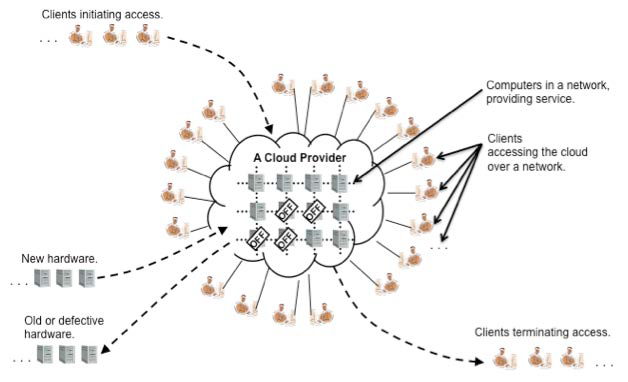
\includegraphics[width=0.4\textwidth]{Images/ConsumerView}
	\caption{Konsumenten Sichtweise \cite{Badger}}
	\label{ConsumerView}
\end{figure}


Alle Kategorien von Cloud-Computing können sogenannte Sicherheitsperimeter verwenden. Diese Regeln den Zugriff auf die Ressource.
In unseren Beispielen kann ein Klient, der sich außerhalb des Sicherheitsperimeter befindet, nur durch einen \glqq boundary controller\grqq
Zugriff zum Netzwerk erlangen.

\subsubsection{Lokale Private Cloud}

Wie in \textbf{Abbildung \ref{PrivateCloud}} zu sehen, befindet sich eine Private Cloud innerhalb der Organisation.
Klienten, die sich innerhalb des Sicherheitsperimeters befinden, können sich mit der Privaten Cloud verbinden. 
Klienten von außerhalb, können eine Verbindung durch den \glqq boundary controller\grqq aufbauen. Dieser Sicherheitsperimeter ist in diesem
Fall optional und wird von dem Konsumenten verwaltet.

\begin{figure}[H]
    \centering
	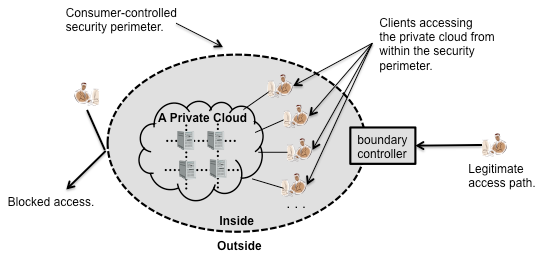
\includegraphics[width=0.4\textwidth]{Images/On-sitePrivateCloud}
	\caption{Private Cloud \cite{Badger}}
	\label{PrivateCloud}
\end{figure}

Die Verwaltung der Cloud wird vom Konsumenten übernommen. Dieser muss die Cloud so einstellen, dass die Arbeitslast zwischen verschiedenen
Maschinen verteilt werden kann, um die Ressourcen optimal nutzen zu können. Außerdem sollten redundante Kopien der Daten auf verschiedenen Maschinen 
gespeichert werden. Dies hat den Vorteil, dass bei einem Serverausfall der Klient auf eine andere Maschine weitergeleitet werden kann.
Außerdem muss der Konsument sicherstellen, dass wichtige Daten wie z.B. Lohnabrechnungen nicht von allen Klienten zugegriffen werden können,
da verschiedenen Daten auf einer Maschine verarbeitet werden können. Der Nachteil von Privaten Clouds ist, dass es hohe Anschaffungskosten, wie z.B. 
das Anschaffen von neuen Daten Zentren, gibt. Außerdem müssen bei z.B. steigenden Zugriffszahlen, neue Hardware vom Konsumenten bereitgestellt werden. 
Dies verringert Flexibilität des Konsumenten.

\subsubsection{Ausgelagerte Private Cloud}

Bei der ausgelagerten Privaten Cloud, wird die Cloud zu einem Provider verlagert. Dieser separiert das Organisationsnetzwerk
von seinem \glqq öffentlichen\grqq Netzwerk, wie in \textbf{Abbildung \ref{OutSourcedPrivateCloud}} zu sehen ist. Das Netzwerk wird vom Provider
durch einen Sicherheitsperimeter geschützt. Der Provider muss dabei sicherstellen, dass die Sicherheitsanforderungen des Konsumenten erfüllt werden. 
Der Konsument kann ebenfalls einen Sicherheitsperimeter in seiner Organisation installieren, um den Zugriff zur Cloud zu regeln.
Die beiden Perimeter werden dann durch einen Kommunikationskanal verbunden und Klienten können dann nur über diesen Kanal auf Daten der Cloud zugreifen.

\begin{figure}[H]
    \centering
	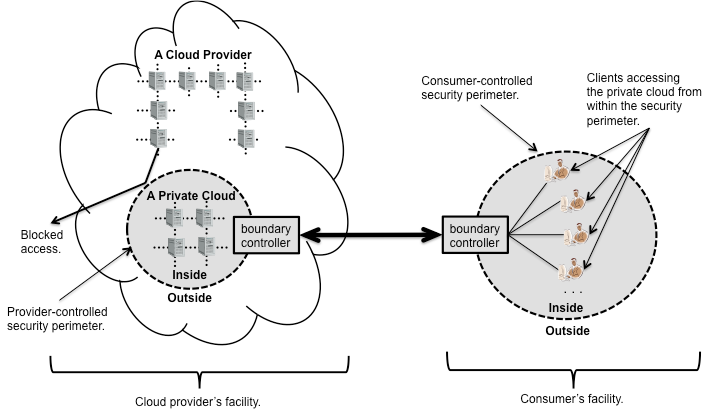
\includegraphics[width=0.4\textwidth]{Images/OutSourcedPrivateCloud}
	\caption{Ausgelagerte Private Cloud \cite{Badger}}
	\label{OutSourcedPrivateCloud}
\end{figure}

Der Konsument ist in diesem Fall von der Netzwerkverfügbarkeit und -geschwindigkeit des Providers abhängig, kann die Geschwindigkeit aber durch Sondertarife erhöhen.
Der Provider muss außerdem sicherstellen, dass die Arbeitslast auf den verschiedenen Maschinen innerhalb des Perimeters verteilt wird und sich die Daten 
nicht mit den Daten von anderen Organisationen, außerhalb des Perimeters, vermischen.
Der Vorteil dieser Architektur ist es, dass der Konsument keine eigenen Ressourcen mehr anschaffen muss und diese beim Provider mieten kann.
Eine Erhöhung der verfügbaren Ressourcen kann jedoch vom Provider nur manuell geschehen, sofern dieser über genug Ressourcen verfügt. 



\subsubsection{Lokale Community Cloud}

Bei der Lokalen Community Cloud teilen mehrere Organisationen ihre Ressourcen und Daten. Alle Organisation stellen und/oder konsumieren Cloud Services.
Dabei muss mindestens eine Organisation solche Services zur Verfügung stellen. Somit ist mindestens eine Organisation, sowohl Provider als auch Konsument.
Sollte jede Organisation einen Sicherheitsperimeter installieren, werden die einzelnen Organisationen durch Kommunikationskanäle zwischen den \glqq boundary controller\grqq verbunden.
Organisationen können außerdem einen weiteren Sicherheitsperimeter einrichten, um die lokalen Cloud Ressourcen von den lokalen Ressourcen zu trennen.

\begin{figure}[H]
    \centering
	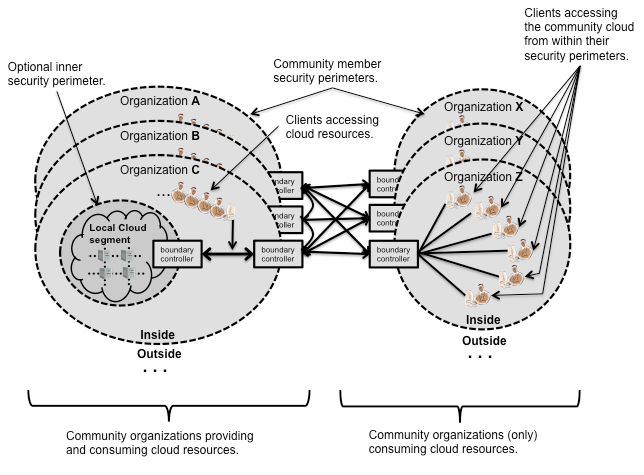
\includegraphics[width=0.4\textwidth]{Images/On-siteCommunityCloud}
	\caption{Lokale Community Cloud \cite{Badger}}
	\label{On-siteCommunityCloud}
\end{figure}

Für die Verwendung der lokalen Community Cloud wird eine komplexe Sicherheitsauthentifizierung benötigt. Jede Organisation der Community muss einen Zugriff bieten und erhalten.
Außerdem müssen die Kommunikationskanäle geschützt und bei der Verwendung des öffentliche Internet Kryptographie verwenden werden. Die einzelnen Kommunikationskanäle zwischen den Teilnehmern 
können verschiedene Level der Performance, Sicherheit und Zuverlässigkeit bereitstellen, abhängig von den Ansprüchen der Teilnehmenden Organisationen. Die Sicherheit der einzelnen Clouds hängt 
hierbei von den den Sicherheitsperimeter der einzelnen Organisationen ab. Ein großer Nachteil dieser Methode sind die hohen Kosten der einzelnen Provider, die Ressourcen 
anschaffen und Services konfigurieren müssen. Die Konsumenten hingegen zahlen nur die Mietkosten der für die Verwendungen der einzelnen Clouds. Ein weiterer Nachteil ist, dass 
die Ressourcen lokal bereitgestellt werden und somit limitiert sind. Wodurch die Flexibilität der einzelnen Organisationen sinkt.


\subsubsection{Ausgelagerte Community Cloud}

Bei der Ausgelagerten Community Cloud verhält es sich ähnlich zu der Ausgelagerten Privaten Cloud, wie in \textbf{Abbildung \ref{OutSourcedCommunityCloud}} zu sehen ist.
Um die Serverseitige Verantwortung kümmert sich hier der Provider, der ein Sicherheitsperimeter installiert und verwaltet. Dabei sorgt der Provider dafür, dass sich 
die Community Ressourcen und die Cloud Provider Ressourcen, die sich außerhalb des Perimeters befinden, nicht vermischen. Ein wesentlicher Unterschied zur Ausgelagerten Privaten Cloud
besteht darin, dass der Cloud Provider möglicherweise eine Freigaberichtlinie zwischen den teilnehmenden Unternehmen der Community Cloud durchsetzen muss. 
Um den Organisationen der Community Konsumenten eine Verbindung zur Cloud zu ermöglichen, müssen sichere Kommunikationskanäle zwischen den einzelnen Organisationen und 
dem Provider installiert werden. 

\begin{figure}[H]
    \centering
	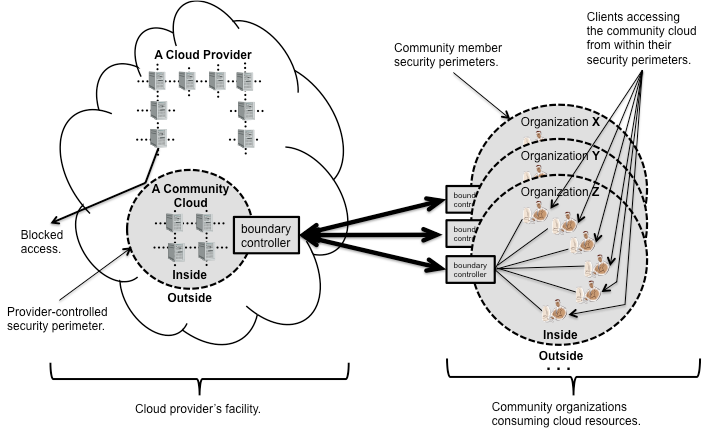
\includegraphics[width=0.4\textwidth]{Images/OutSourcedCommunityCloud}
	\caption{Ausgelagerte Community Cloud \cite{Badger}}
	\label{OutSourcedCommunityCloud}
\end{figure}


\subsubsection{Public Cloud}

Die Public Cloud, die in \textbf{Abbildung \ref{PublicCloud}} zu sehen ist, verhält sich recht ähnlich zu \textbf{Abbildung \ref{ConsumerView}}.
Außer das der Konsument einen eigenen Sicherheitsperimeter installiert, um den Zugriff zur Cloud zu regeln.

 
\begin{figure}[H]
    \centering
	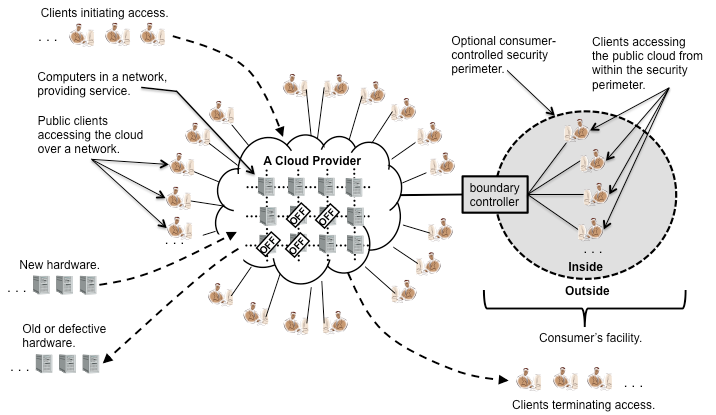
\includegraphics[width=0.4\textwidth]{Images/PublicCloud}
	\caption{Public Cloud \cite{Badger}}
	\label{PublicCloud}
\end{figure}

In diesem Szenario verbindet sich der Konsument über das öffentliche Internet, sodass die Verbindungsqualität und -zuverlässigkeit zur Cloud
von dem Internet Provider, dem DNS Server und der Router Infrastruktur abhängt. Die Arbeitslast oder Ressourcen eines Konsumenten können zu jeder Zeit
vom Provider migriert werden. Ein großer Vorteil der Public Cloud ist die Kosteneffizient, da Datenzentren an Standorten verwendet werden können, die für den Konsumenten am günstigen sind.
Ein Beispiel dafür wäre, das die Arbeitslast eines Deutschen Unternehmens in einem Deutschen Datenzentrum verarbeitet und somit die Performance verbessert wird (geringe Übertragungswege).
Dies wird aber meist nicht von Provider versichert. Die Arbeitslast kann an verschiedenen Standorten (Europa, USA, China usw.) verarbeitet werden, außer der Provider bietet eine
Standortbeschränkung an. Ein großes Problem der Public Cloud ist es, dass eine Maschine die Daten von mehreren Konsumenten verarbeiten kann und somit ein Sicherheitsrisiko entstehen kann.
Außerdem haben die Konsumenten keine Möglichkeit die Einsicht ihrer Daten zu überwachen oder eine Authentifizierung für ihre Daten einzurichten. Da große Anbieter meist eine Monitoring für die
Daten durchführen, um die Tatsächliche Datennutzung zu ermitteln und den Konsumenten diese dann in Rechnung zu stellen, ist diese Methode nicht für sensible oder wichtige Daten geeignet.
Außerdem kann der Konsument nie sicher sein, ob sein Daten auch gelöscht werden, wenn er den Vertrag kündigt. 
Ein großer Vorteil der Public Cloud ist die Uneingeschränktheit in Hinsicht des Standortes und der Größe. D.h. die Größe der zur Verfügung gestellten Ressourcen lässt sich 
meist \glqq uneingeschränkt\grqq erhöhen oder vermindern.

Bekannte Public Cloud Provider sind Amazon Web Services (AWS) und Microsoft Azure. 


% \subsubsection{Hybrid Cloud}
% Eine Hybrid Cloud besteht aus mindestens zwei oder mehreren Privaten, Community oder Public Clouds.
% \begin{figure}[H]
%     \centering
% 	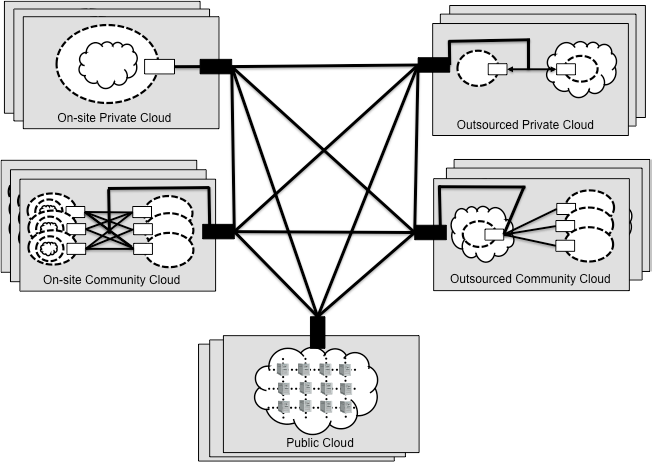
\includegraphics[width=0.4\textwidth]{Images/HybridCloud}
% 	\caption{Hybrid Cloud \cite{Badger}}
% 	\label{HybridCloud}
% \end{figure}

\subsection{Architekturen der Dienstmodelle}

In diesem Abschnitt werden die Architekturen der drei Dienstmodelle SaaS, PaaS, IaaS beschrieben.

\subsubsection{SaaS}\label{SaaS Architektur}

\begin{figure}[H]
    \centering
	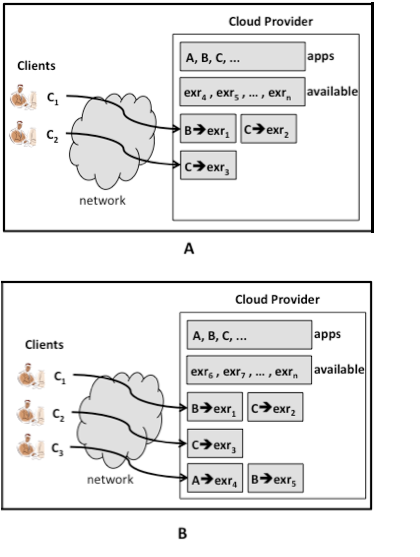
\includegraphics[width=0.4\textwidth]{Images/SaaSInteraction}
	\caption{SaaS Interaktion \cite{Badger}}
	\label{SaaSInteraction}
\end{figure}
Wie bereits in Abschnitt \ref{IaaS} beschrieben, stellt der Provider den Klienten Anwendungen (\glqq Apps\grqq) zu Verfügung.
Diese Anwendungen können dann über das öffentliche Internet (Webseiten) aufgerufen werden.
Wie in \textbf{Abbildung \ref{SaaSInteraction}.A} zu sehen ist, kann ein Provider mehrere Apps anbieten und ausführen.
Er hat dabei eine gewisse Anzahl an \glqq Execution Ressources\grqq (exr) zur Verfügung. 
Dabei wird den Klienten bei jedem starten einer Anwendung eine exr zugewiesen. Sollten neue Klienten hinzukommen, werden ihm verbleibende Ressourcen (exr) zugewiesen. 

\begin{figure}[H]
    \centering
	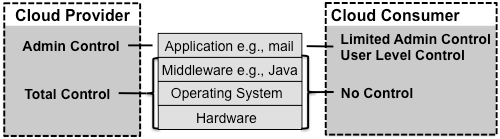
\includegraphics[width=0.4\textwidth]{Images/SaaSControl}
	\caption{SaaS Kontrollverteilung \cite{Badger}}
	\label{SaaSControl}
\end{figure}

\textbf{Abbildung \ref{SaaSControl}} zeigt, wie die Kontroll- und Managementverantwortung zwischen den Provider und den Konsumenten verteilt wird.
Bei Software as a Service hat der Konsument nur die Kontrolle auf der Benutzerebene, d.h. dieser kann Benutzerverwalten wie z.B. Benutzer hinzufügen.
Der Provider hingegen verfügt die totale Kontrolle über alle Bereiche. Diese muss ist Verantwortlich für das Erstellen, konfigurieren und Verwalten der Anwendungen, 
sodass der Konsument diesen Service nutzen kann.
Bei der Middleware Schicht kann der Provider sowohl über die Software Bibliotheken, als auch Datenbankenservices entscheiden, der Konsument hat darauf keinen Einfluss.
Das selbe gilt bei der Wahl des Betriebssystems und der Hardware, bei der der Konsument keinen Einfluss hat.

\subsubsection*{Vorteile von SaaS}

Im Vergleich zu traditionellen Computing- und Softwareverteilungslösungen bieten SaaS-Clouds Skalierbarkeit und verlagern zudem die Belastungen vom Konsumenten zum Provider.
Die Vorteile eines solchen Services sind, dass für öffentliche und ausgelagerten Szenarien, sich der Großteil der von einer Anwendung verwalteten Daten auf den Softwareverteilungslösungen
des Cloud-Providers befinden. Der Provider kann diese Daten dezentral und Redundant speichern, sodass ein Verlust von Daten unwahrscheinlich wird. Außerdem bieten SaaS-Provider
ein professionelles Management System an, dass z.B. Compilance-Check (Datenschutz), Security-Scanning (Virenprüfung), Backup und Disaster Recovery unterstützt.


\subsubsection{Funktionsweise von SaaS}

Wie bereits erwähnt wird bei Starten einer Anwendung von einem Nutzer ein Prozess (exr) gestartet. Dabei haben die Provider meist eine statische oder eine dynamische
Lösung, um die Anwendung zu betreiben, wie \textbf{Abbildung \ref{SaaSM1}} zeigt.

\begin{figure}[H]
    \centering
	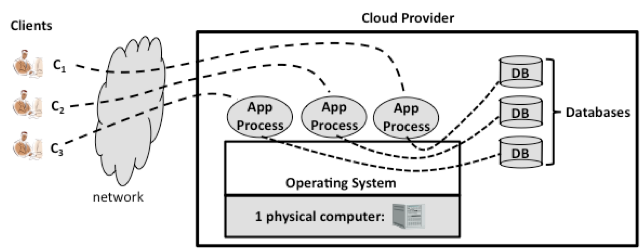
\includegraphics[width=0.4\textwidth]{Images/SaaSM1}
	\caption{Möglichkeit 1 \cite{Badger}}
	\label{SaaSM1}
\end{figure}

In diesem Szenario wird eine aktive Kopie der Anwendung für jeden Benutzer gestartet. Jede Anwendung betreibt dabei ein eigenes Datenbanksystem, indem die Daten der Benutzer gespeichert werden.
Somit besitzt jeder Klient eine eigene Kopie der Daten. Die einzelnen Kopien der Anwendung, der Datenbanksysteme und die Separierung der Benutzer wird durch das Betriebssystem ermöglicht.
Ein großer Nachteil dieses Szenarios ist es, dass hohe Kosten für das Betreiben und Synchronisieren der einzelnen Datenbanksystemen entstehen.


\begin{figure}[H]
    \centering
	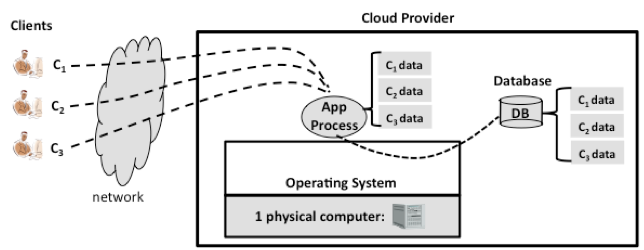
\includegraphics[width=0.4\textwidth]{Images/SaaSM2}
	\caption{Möglichkeit 2 \cite{Badger}}
	\label{SaaSM2}
\end{figure}

Beim statischen Szenario (\textbf{Abbildung \ref{SaaSM2}}) wird die Anwendung vom Provider so implementiert, sodass mehrere Klienten gleichzeitig daran Arbeiten können und die Daten in nur einem Datenbanksystem gespeichert werden. 
Dies hat den Vorteil das die Kosten für den Provider gesenkt werden, da nur noch eine Anwendung betrieben wird.
Die Anwendung selbst, muss dafür aber die Daten mehrerer Klienten gleichzeitig verarbeiten und trotzdem sicherstellen, dass die Sicherheit der Daten gewährleistet ist.   

\subsubsection{Paas}

Der Unterschied von Platform as a Service zu Software as a Service ist, das Konsumenten die Möglichkeit haben, eigene Anwendungen bei dem Cloud Provider 

\begin{figure}[H]
    \centering
	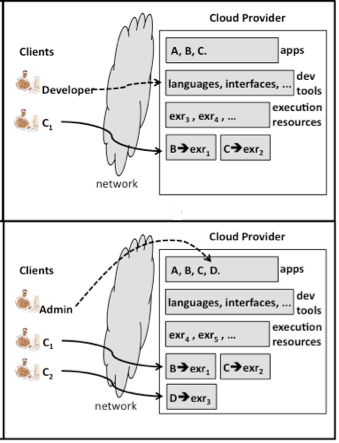
\includegraphics[width=0.4\textwidth]{Images/PaaSInteraction}
	\caption{PaaS Interaktion \cite{Badger}}
	\label{PaaSInteration}
\end{figure}

aaaaaa
\begin{figure}[H]
    \centering
	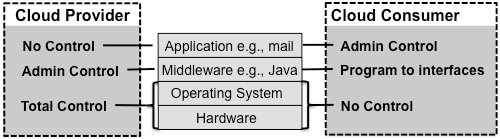
\includegraphics[width=0.4\textwidth]{Images/PaaSControl}
	\caption{PaaS Kontrollverteilung \cite{Badger}}
	\label{PaaSControl}
\end{figure}

\subsubsection{IaaS}
aaa
\begin{figure}[H]
    \centering
	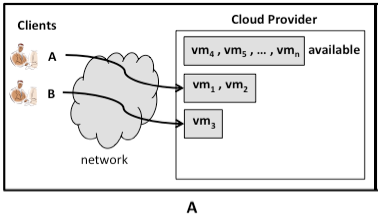
\includegraphics[width=0.4\textwidth]{Images/IaaSInteraction}
	\caption{IaaS Interaktion \cite{Badger}}
	\label{IaaSInteraction}
\end{figure}

aaa
\begin{figure}[H]
    \centering
	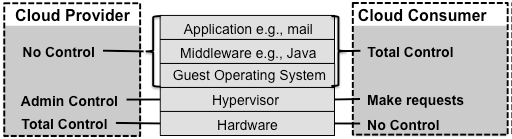
\includegraphics[width=0.4\textwidth]{Images/IaaSControl}
	\caption{IaaS Kontrollverteilung \cite{Badger}}
	\label{IaaSControl}
\end{figure}

\subsection{Logische Sichtweise}
aaaaaaaaa
\begin{figure}[H]
    \centering
	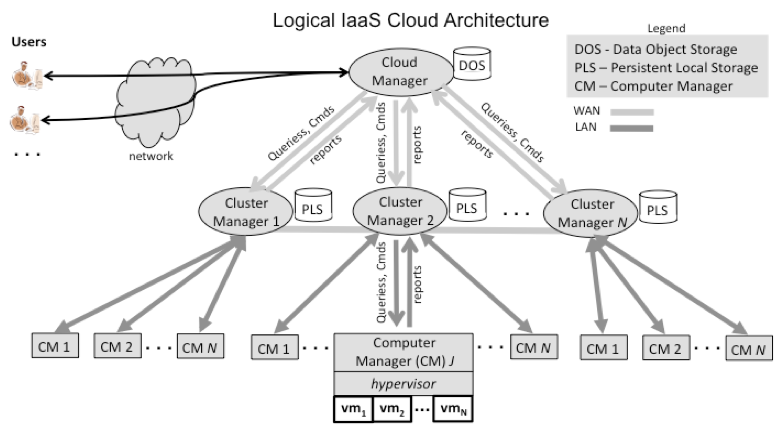
\includegraphics[width=0.4\textwidth]{Images/IaaSLogic}
	\caption{IaaS Logische Sichtweise \cite{Badger}}
	\label{IaaSLogic}
\end{figure}

% \subsection{Management}
%\pagebreak
\section{Abgrenzung zu Grid Computing}
Der Ansatz -- die Infrastruktur, Rechenleistung sowie Anwendungen oder Speicherplatz über ein Netzwerk für verschiedene Zwecke zur Verfügung zu stellen -- ist kein neuer.
Diese Idee, oder zumindest eine ähnliche, entstand schon vor mehreren Jahren mit dem Begriff \textbf{Grid Computing}.

Im folgenden Abschnitt werden einige Aspekte erläutert, die den Unterschied zwischen Cloud Computing und Grid Computing verdeutlichen.
 
\subsection{Der Begriff \glqq Grid Computing\grqq}
In \cite{grid-checklist} schlägt der Autor eine 3-Punkte-Checkliste vor, anhand deren sich ein Grid-System identifizieren lässt. Demnach ist Grid ein System, das:
\begin{enumerate}
  \item Ressourcen koordiniert, die keiner zentralisierten Kontrolle unterliegen
  \item dabei offene und allgemeine Standardprotokolle und Schnittstellen verwendet
  \item um nicht-triviale \glqq Quality of Services\grqq{} zu liefern
\end{enumerate}

Cloud Computing überschneidet sich nicht nur mit Grid Computing, es ist in der Tat aus Grid Computing entstanden und bildet dessen Rückgrad auf dem seine Infrastruktur aufbaut\cite{360-degree-compared}.

Das spezielle Problem, das dem Konzept des Grids in Wirklichkeit zugrunde liegt,
ist die koordinierte gemeinsame Nutzung von Ressourcen und das Lösen von Problemen
in einer dynamischen institutionsübergreifenden virtuellen Organisation.
Dabei ist mit \glqq gemeinsamer Nutzung\grqq{} der direkte Zugang zu Computern, Software, Daten und anderen Ressourcen,
die für das Lösen von Problemen in industriellen, wissenschaftlichen und technischen Bereichen benötigt werden, zu verstehen.
Das Teilen der Ressourcen beinhaltet klar definierte Regeln, die notwendigerweise stark kontrolliert werden.
Was geteilt werden kann, wer teilen darf und unter welchen Bedingungen geteilt werden darf ist dabei klar und sorgfältig definiert.
Eine Gruppe von Individuen und/oder Institutionen, die durch solche Regeln definiert sind,
bilden die sogenannten \textbf{Virtuellen Organisationen}.\cite{anatomy-of-grid}

\subsection{Anwendungsbereich}

Hier soll es darum gehen, wo hauptsächlich Grid bzw. Cloud Verwendung findet. Z.B. Grid: forschung, rechenintensive Applicationen; Cloud: kommerzielle Zwecke etc.
Bei Anwendungen von Cloud Computing nicht ins Detail gehen, da es schon ein extra Kapitel gibt.

\subsection{Geschäftsmodell}
Typischerweise ist das Geschäftsmodell der Grids (zumindest im akademischen Bereich) projektorientiert und die Anwender oder die Community hat eine bestimmte Anzahl an Serviceeinheiten, die verbraucht werden können\cite{360-degree-compared}.  
Dieses Konzept wird beispielsweise von XSEDE (Extreme Science and Engineering Discovery Environment) -- einem Anbieter von digitalen Dienstleistungen wie Supercomputern -- verwendet\cite{xsede}.
Wenn eine Institution mit ihren eigenen Ressourcen einem solchen Netzwerk beitritt stellt sie diese zur Nutzung für die Community bereit und kann aber dafür auf die Ressourcen der anderen zugreifen\cite{360-degree-compared}.

\subsection{Architektur}
Die Grid-Netze konzentrieren sich auf die Integration vorhandener Ressourcen mit ihrer Hardware, Betriebssystemen, lokalem Ressourcenmanagement und der Sicherheitsinfrastruktur.
Um die Entdeckung sowie die gemeinsame Nutzung von diesen Ressourcen in den sogenannten \glqq Virtuellen Organisationen\grqq{} zu ermöglichen, stellen Grids eine Menge von Standardprotokollen, Middleware, Toolkits sowie Diensten, die auf diesen Protokollen aufbauen, bereit.
Da Ressourcen von verschiedene administrativen Domänen sein können und somit ihre eigene Verwendungsregeln, andere Hard- oder Softwarekonfiguration haben können, stellt die Interoperabilität und Sicherheit das Hauptanliegen für die Gridinfrastruktur dar.\cite{360-degree-compared}

\begin{figure}[ht]
	\centering
  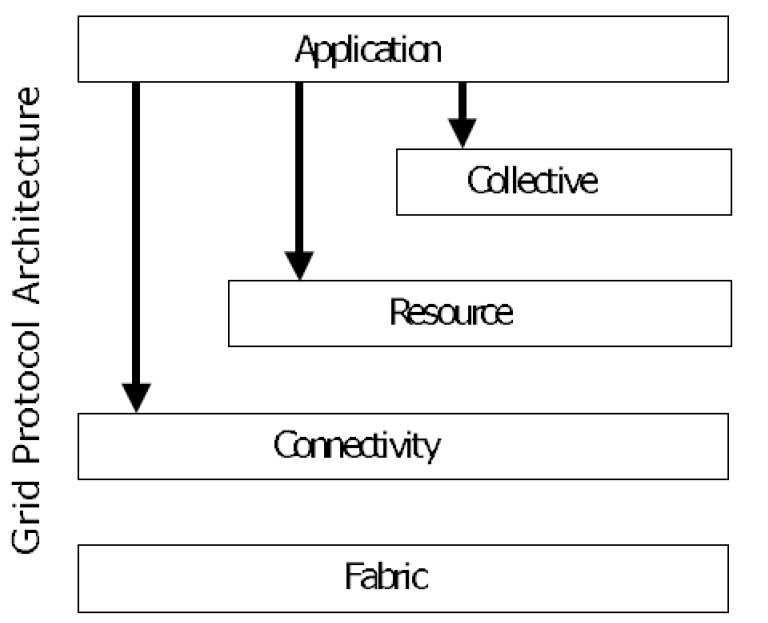
\includegraphics[width=0.5\textwidth]{res/grid-protocol-arch.jpg}
	\caption{Grid protocol architecture\cite{360-degree-compared}}
	\label{gpa}
\end{figure}
\hlred{Die Ressourcen einer virtuellen Organisation können geographisch verteilt sein.}\todo{Zitat finden}

\subsection{Ressourcenverwaltung}
Während Grid Computing versucht Ressourcen zu bündeln, die innerhalb unterschiedlicher Organisationen sich befinden, bietet Cloud Computing diese meistens innerhalb einer einzelnen Organisation. Dies vereinfacht unter anderem solche Aspekte wie Sicherheit, Verfügbarkeit und Heterogenität\cite{comp-cloud-grid-cluster-virt}.

Virtualisierung, Compute Model (Batch-scheduled compute model bei Grid vs Cloud etc.) usw.

\subsection{Fazit}
\hlred{Während Cloud Computing hauptsächlich Lösungen für verschiedene webbasierte Businessfälle bietet, wird Grid Computing dagegen mehr in wissenschaftlichen Projekten bei rechenintensiven Aufgaben eingesetzt.
Grid Computing systems are not intended to be used in business purposes. e.i. there is no business model behind it. The users or organisations who want to make use of Grid Computing simply join a VO and start consuming
Aus Benutzersicht werden Ressourcen bei Cloud Computing zentral verwaltet.
Der Benutzer kann, im Web, vom Cloud Provider zur Verfügung gestellte Schnittstelle verwenden,
um Ressourcen bei Bedarf hinzuzufügen oder zu entfernen.
Grid Computing ist in dieser Hinsicht dezentralisiert. 
Die Ressourcen können sich in unterschiedlichen virtuellen Organisationen befinden.} 

[Wie sieht es für die Zukunft aus?]

\hl{Wird man in der Zukunft komplett auf Grid Computing verzichten können und stattdessen auf Cloud Computing Lösungen zugreifen?}

\section{Fazit}
Es lässt sich festhalten, dass Cloud Computing überall dort sinnvoll ist, wo skalierbare Rechenressourcen gebraucht werden und eine gewisse Anzahl an Benutzern von überall auf diese zugreifen können soll.



%\subsubsection{Subsubsection Heading Here}
%Subsubsection text here.


% An example of a floating figure using the graphicx package.
% Note that \label must occur AFTER (or within) \caption.
% For figures, \caption should occur after the \includegraphics.
% Note that IEEEtran v1.7 and later has special internal code that
% is designed to preserve the operation of \label within \caption
% even when the captionsoff option is in effect. However, because
% of issues like this, it may be the safest practice to put all your
% \label just after \caption rather than within \caption{}.
%
% Reminder: the "draftcls" or "draftclsnofoot", not "draft", class
% option should be used if it is desired that the figures are to be
% displayed while in draft mode.
%
%\begin{figure}[!t]
%\centering
%\includegraphics[width=2.5in]{myfigure}
% where an .eps filename suffix will be assumed under latex, 
% and a .pdf suffix will be assumed for pdflatex; or what has been declared
% via \DeclareGraphicsExtensions.
%\caption{Simulation results for the network.}
%\label{fig_sim}
%\end{figure}

% Note that the IEEE typically puts floats only at the top, even when this
% results in a large percentage of a column being occupied by floats.


% An example of a double column floating figure using two subfigures.
% (The subfig.sty package must be loaded for this to work.)
% The subfigure \label commands are set within each subfloat command,
% and the \label for the overall figure must come after \caption.
% \hfil is used as a separator to get equal spacing.
% Watch out that the combined width of all the subfigures on a 
% line do not exceed the text width or a line break will occur.
%
%\begin{figure*}[!t]
%\centering
%\subfloat[Case I]{\includegraphics[width=2.5in]{box}%
%\label{fig_first_case}}
%\hfil
%\subfloat[Case II]{\includegraphics[width=2.5in]{box}%
%\label{fig_second_case}}
%\caption{Simulation results for the network.}
%\label{fig_sim}
%\end{figure*}
%
% Note that often IEEE papers with subfigures do not employ subfigure
% captions (using the optional argument to \subfloat[]), but instead will
% reference/describe all of them (a), (b), etc., within the main caption.
% Be aware that for subfig.sty to generate the (a), (b), etc., subfigure
% labels, the optional argument to \subfloat must be present. If a
% subcaption is not desired, just leave its contents blank,
% e.g., \subfloat[].


% An example of a floating table. Note that, for IEEE style tables, the
% \caption command should come BEFORE the table and, given that table
% captions serve much like titles, are usually capitalized except for words
% such as a, an, and, as, at, but, by, for, in, nor, of, on, or, the, to
% and up, which are usually not capitalized unless they are the first or
% last word of the caption. Table text will default to \footnotesize as
% the IEEE normally uses this smaller font for tables.
% The \label must come after \caption as always.
%
%\begin{table}[!t]
%% increase table row spacing, adjust to taste
%\renewcommand{\arraystretch}{1.3}
% if using array.sty, it might be a good idea to tweak the value of
% \extrarowheight as needed to properly center the text within the cells
%\caption{An Example of a Table}
%\label{table_example}
%\centering
%% Some packages, such as MDW tools, offer better commands for making tables
%% than the plain LaTeX2e tabular which is used here.
%\begin{tabular}{|c||c|}
%\hline
%One & Two\\
%\hline
%Three & Four\\
%\hline
%\end{tabular}
%\end{table}


% Note that the IEEE does not put floats in the very first column
% - or typically anywhere on the first page for that matter. Also,
% in-text middle ("here") positioning is typically not used, but it
% is allowed and encouraged for Computer Society conferences (but
% not Computer Society journals). Most IEEE journals/conferences use
% top floats exclusively. 
% Note that, LaTeX2e, unlike IEEE journals/conferences, places
% footnotes above bottom floats. This can be corrected via the
% \fnbelowfloat command of the stfloats package.




%\section{Conclusion}
%The conclusion goes here.\cite{NIST_Definition} \cite{IEEEhowto:kopka}




% conference papers do not normally have an appendix


% trigger a \newpage just before the given reference
% number - used to balance the columns on the last page
% adjust value as needed - may need to be readjusted if
% the document is modified later
%\IEEEtriggeratref{8}
% The "triggered" command can be changed if desired:
%\IEEEtriggercmd{\enlargethispage{-5in}}

% references section

% can use a bibliography generated by BibTeX as a .bbl file
% BibTeX documentation can be easily obtained at:
% http://mirror.ctan.org/biblio/bibtex/contrib/doc/
% The IEEEtran BibTeX style support page is at:
% http://www.michaelshell.org/tex/ieeetran/bibtex/
%\bibliographystyle{IEEEtran}
% argument is your BibTeX string definitions and bibliography database(s)
%\bibliography{IEEEabrv,../bib/paper}
%
% <OR> manually copy in the resultant .bbl file
% set second argument of \begin to the number of references
% (used to reserve space for the reference number labels box)
% \begin{thebibliography}{1}

% \bibitem{IEEEhowto:kopka}
% H.~Kopka and P.~W. Daly, \emph{A Guide to \LaTeX}, 3rd~ed.\hskip 1em plus
%   0.5em minus 0.4em\relax Harlow, England: Addison-Wesley, 1999.

% \end{thebibliography}



\bibliography{swa}
\bibliographystyle{ieeetr}




% that's all folks
\end{document}


